\documentclass[3pt]{article}
\usepackage{amsmath,amsfonts,amssymb}
\usepackage{graphicx}
\usepackage{listings}
\usepackage{enumitem}
\graphicspath{{/Users/diesel/Desktop/}}
\newcommand{\floor}[1]{\lfloor #1 \rfloor}
\usepackage{tabu}

\title{Solution to Homework 2b(CS 553)}
\author{Saptarshi Chatterjee \\
\texttt{CWID: A20413922}
}

\begin{document}
\maketitle

\section{Table 1: Performance evaluation of sort (weak scaling-small dataset) }

\setlength{\parskip}{1.2em}
\setlength{\parindent}{0em}


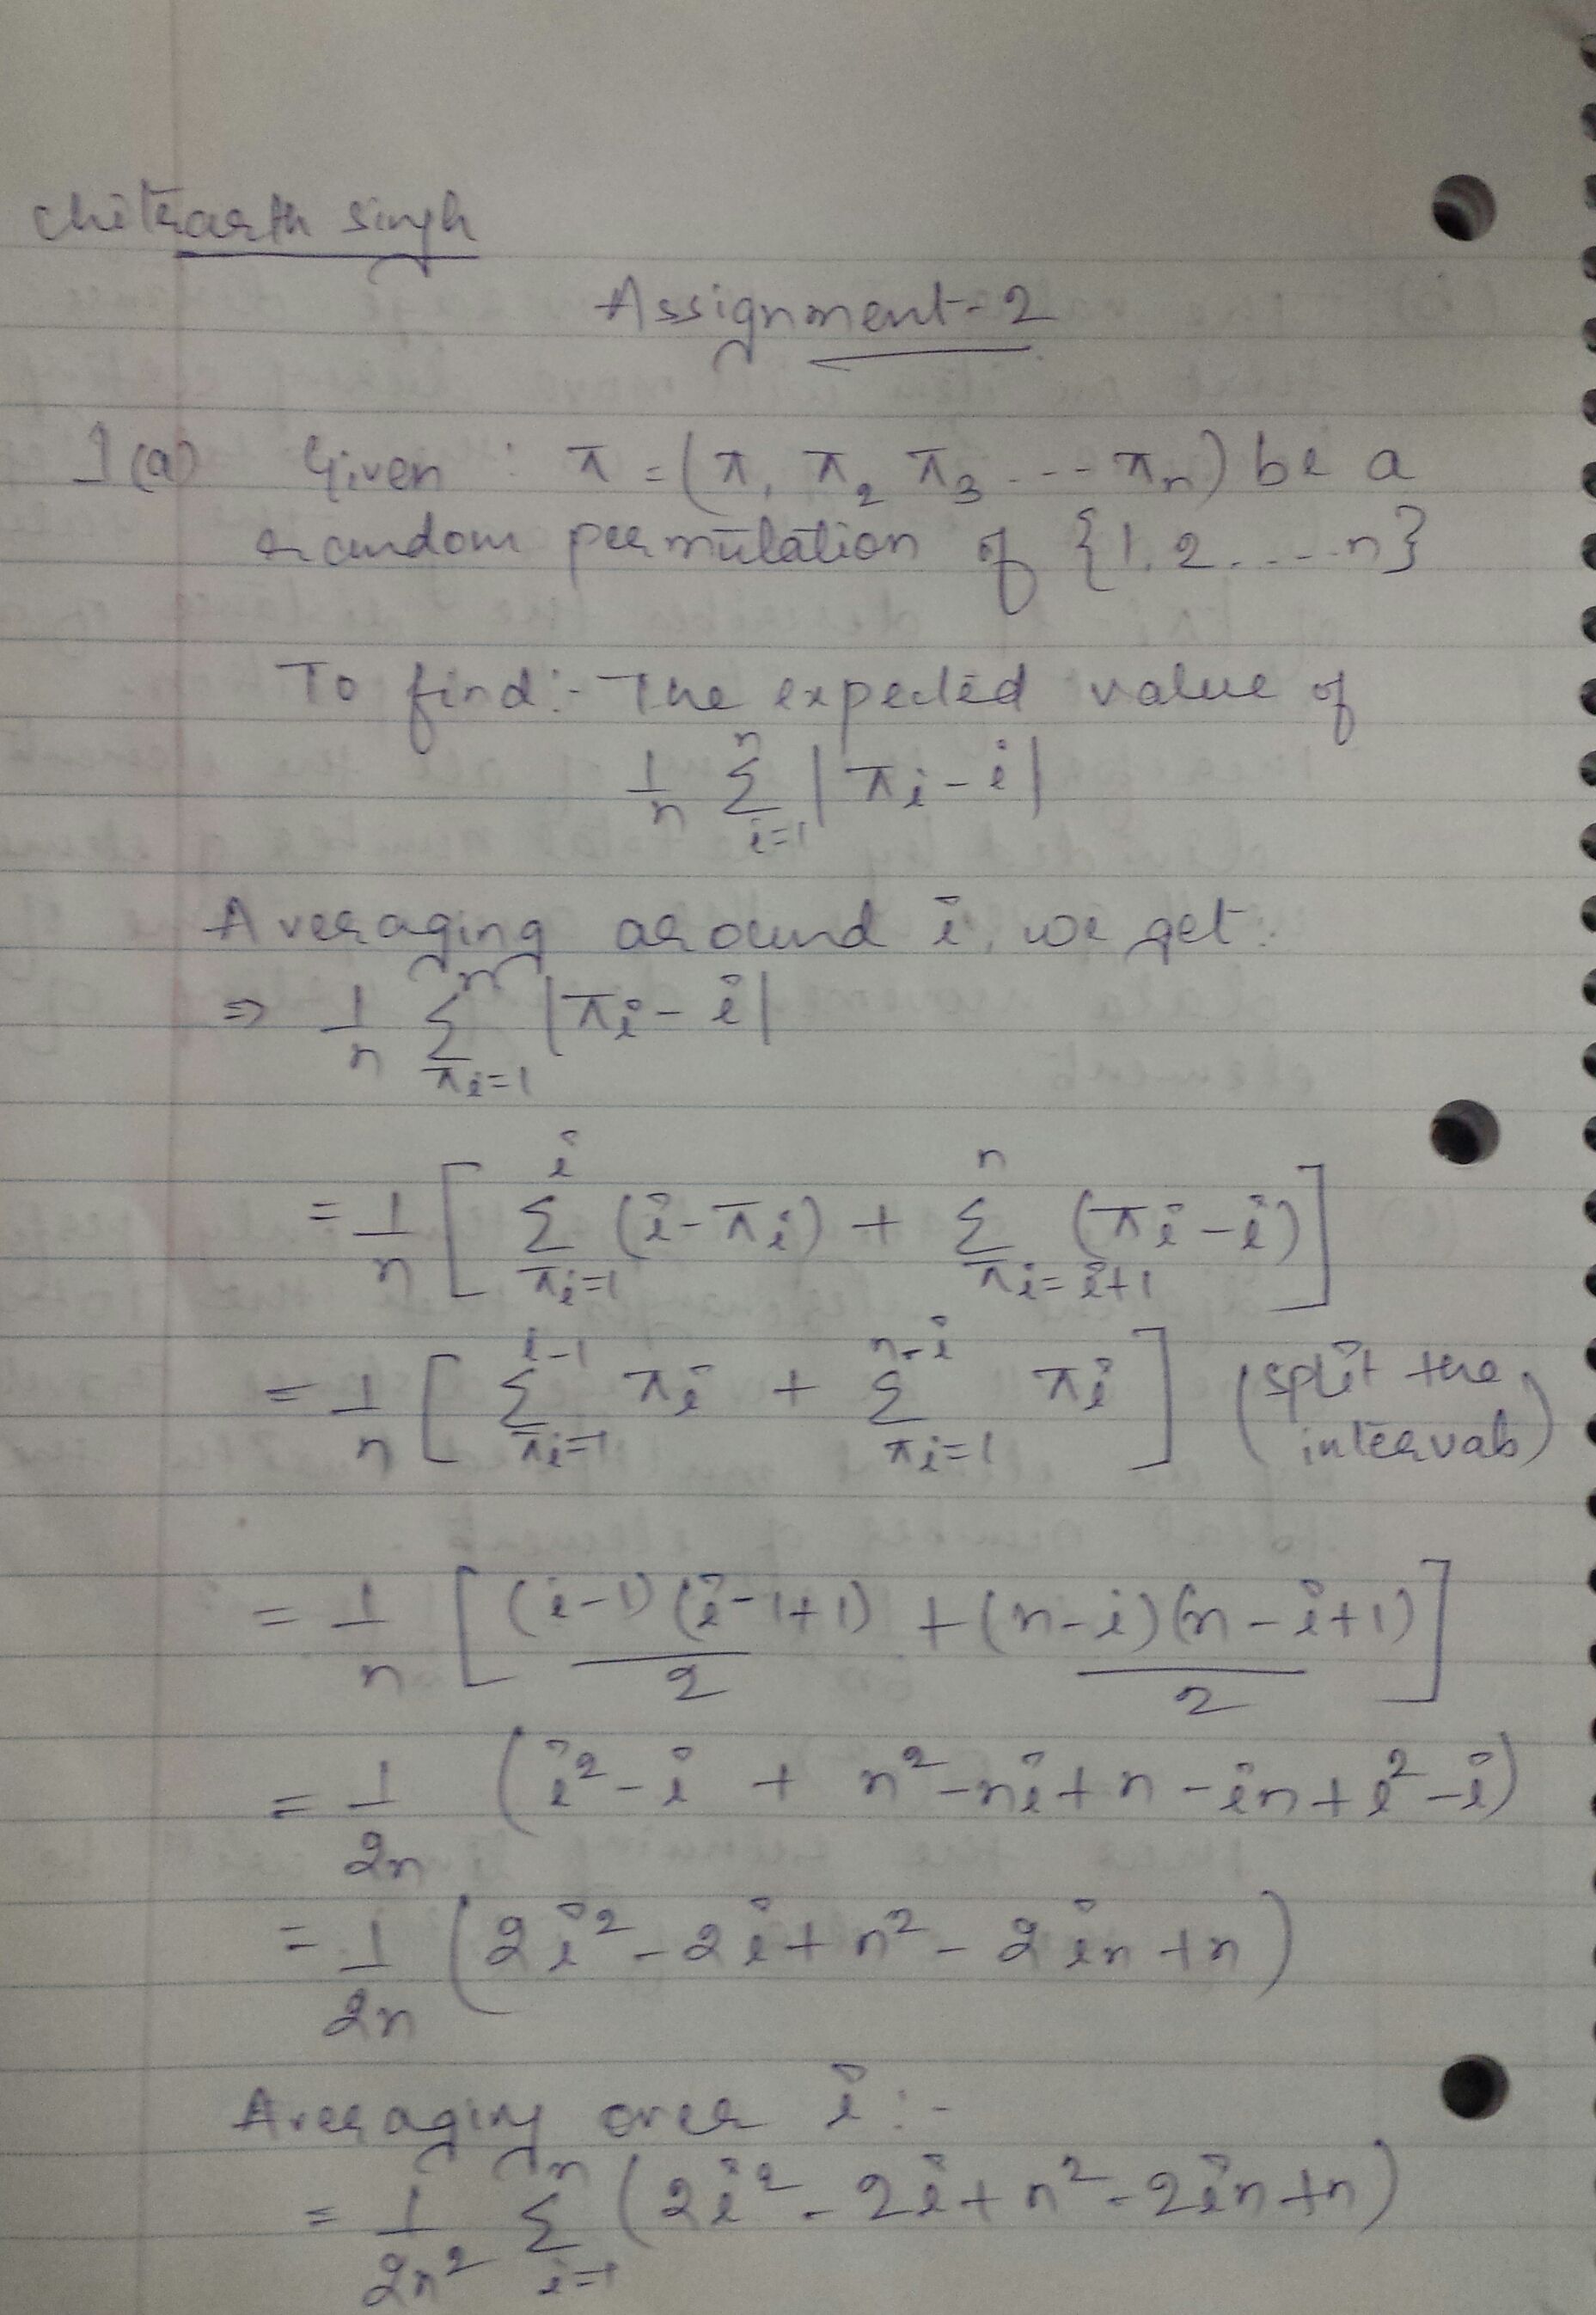
\includegraphics[scale=.5]{1} \\

\textbf{Running Hadoop on Cluster} \\
\\
\includegraphics[scale=.3]{hadoop8Gb} \\

\textbf{Success Output} \\

\includegraphics[scale=.5]{success} \\

\section{Table 2: Performance evaluation of sort (strong scaling-large dataset)}

\setlength{\parskip}{1.2em}
\setlength{\parindent}{0em}


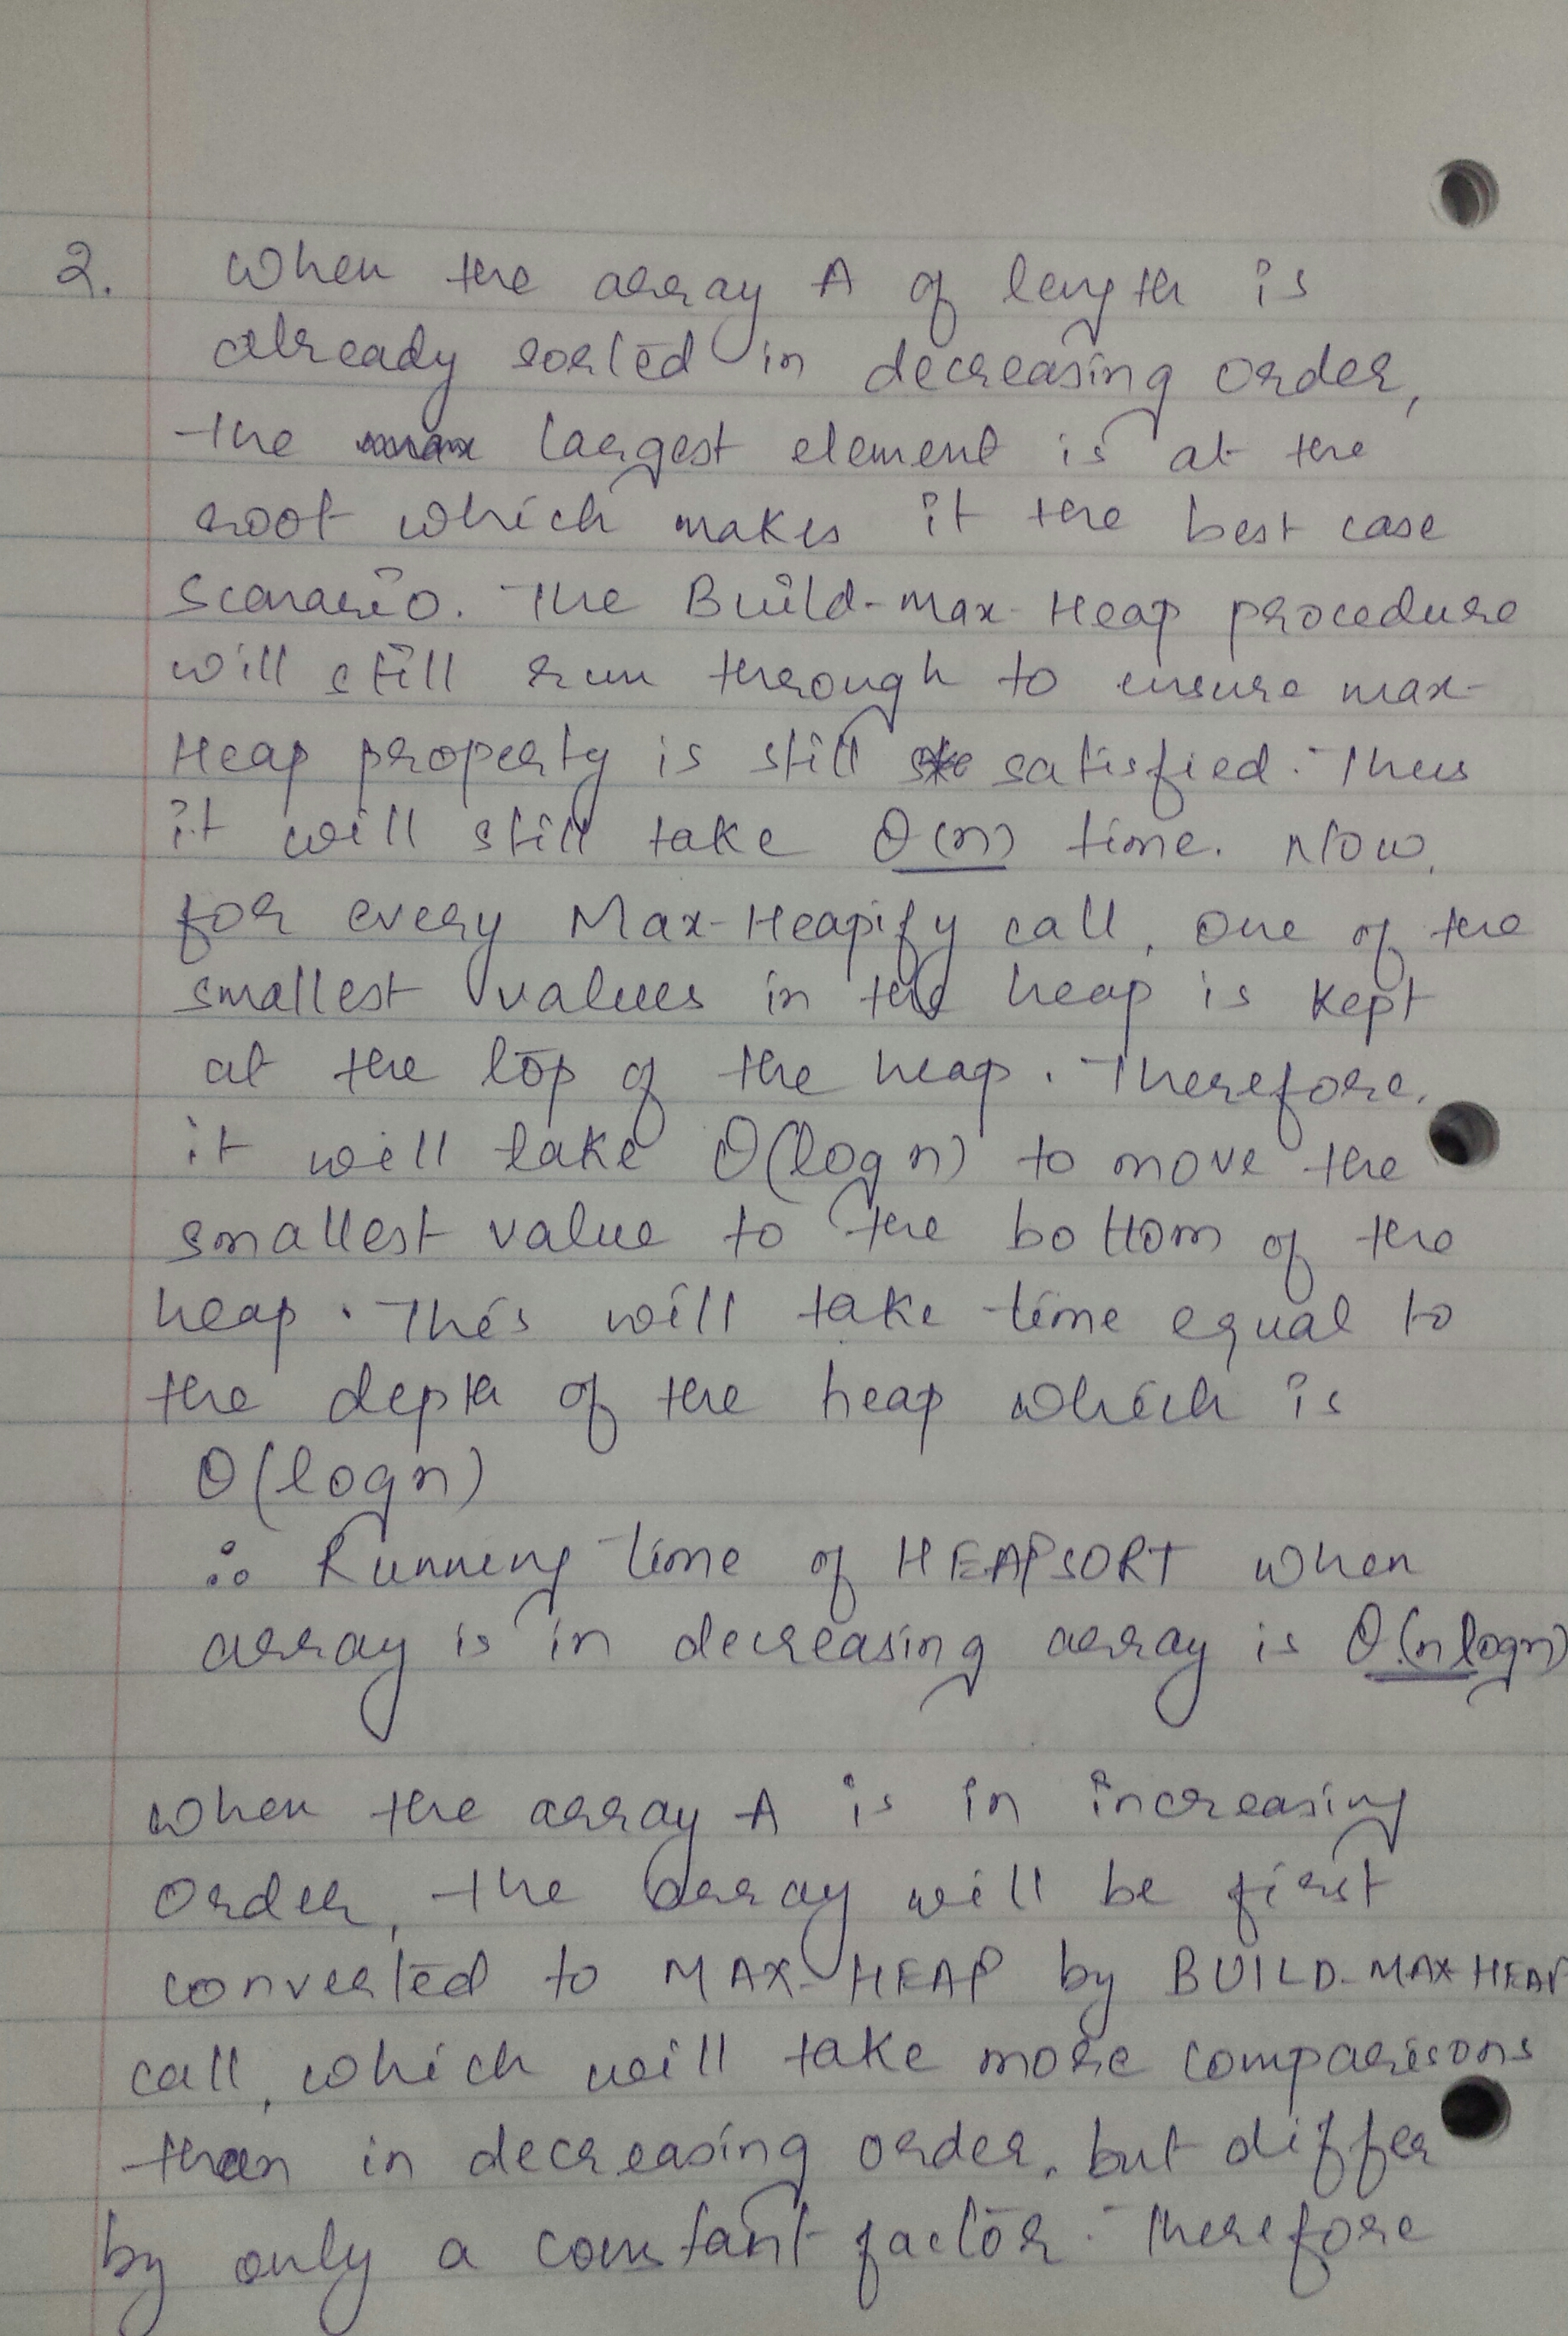
\includegraphics[scale=.5]{2} \\

\textbf{Running with 80GB dataSet} \\

\includegraphics[scale=.4]{80GB} \\

\section{Table 3: Performance evaluation of sort (weak scaling-large dataset)}

\setlength{\parskip}{1.2em}
\setlength{\parindent}{0em}


\includegraphics[scale=.5]{3} \\

\textbf{Spark Run} \\

\includegraphics[scale=.5]{sparkrun} \\


\section{What conclusions can you draw? Which seems to be best at 1 node scale? How about 4 nodes? Can you predict which would be best at 100 node scale? How about 1000 node scales?} 

In the context of high performance computing there are two common notions of scalability: \\
\\
- The first is strong scaling, which is defined as how the solution time varies with the number of processors for a fixed total problem size. \\
\\
~~-The second is weak scaling, which is defined as how the solution time varies with the number of processors for a fixed problem size per processor \\


\textbf{Synopsis}

\begin{itemize}

\item Hadoop  is stores intermediate result in HDFS , so it involves intermediate storage in Disk 
\\
~~ \includegraphics[scale=.5]{hadoop}

\item Spark uses in-memory computation and Uses RDD to speed up execution
\\
~~ \includegraphics[scale=.1]{spark}

\item Spark uses in-memory computation and Uses RDD to speed up execution

\item For small 2GB data set 1VM linux sort provides best performance , as Hadoop and Spark involves overhead for Scheduling and Tracking .

\item For Single node Hadoop and Spark has almost similar efficiency

\item For large DataSets Spark is significantly faster than Hadoop

\item As we increase number of machines the efficiency doesn't increase linearly .

\item For 100 node scale we should get 50-60X speed-up , for 1000 nodes speed up should be 300-400X.

\end{itemize}

\end{document}